\section{Schluss}
\label{sec:schlusswort}

\subsection{Weiteres Vorgehen}

Das in PREN 1 Erarbeitete bildet den Grundstein für das nächste Semester, mit dem Ziel, das Konzept umzusetzen und das Projekt erfolgreich zum Abschluss zu bringen. In PREN 1 konnten schon einige Schwierigkeiten frühzeitig erkannt und grösstenteils ausgeräumt werden. Das Konzept genügt den Anforderungen weitgehend. Für kritische Komponenten stehen Alternativen zur Verfügung. Nun ist es wichtig, die erarbeiteten Pläne zu präzisieren, damit die Konstruktion weiter an Form gewinnt, sodass am Ende vom Modul PREN 2 das voll funktionsfähige \textit{Silisloth} herauskommt, das mehr leistet, als nur kopfüber von einem Seil zu hängen und dabei Ressourcen zu verbrauchen.

\subsection{Lessons Learned}

\begin{description}
\item[Anforderungen] Anforderungen können sich im Verlauf eines Projektes ändern. Betreffend Zugwiderstand des Seils unterscheideten sich zu Beginn die Abschätzungen erheblich vom aufgestellten Parcours, was sich aber aufgrund der später ausgetauschten Laufrollen wieder etwas anglich. Darum ist es nötig, bei wichtigen Parametern (wie etwa dem Gewicht) nicht ans absolute Limit zu gehen, sondern etwas Spielraum einzuberechnen.
\item[Bildverarbeitung] Für die Bildverarbeitung lohnt es sich genügend Zeit in die Recherche zu investieren. Dadurch lassen sich nicht nur weit verbreitete Bildverarbeitungs-Libraries wie OpenCV finden, sondern auch passenden Beispiele dazu.
\item[Dokumentation] Typografisch hochstehende Ergebnisse erreicht man mit \LaTeX, wenn man bereit ist den entsprechenden Aufwand auf sich zu nehmen. Gerade die Darstellung von Tabellen ist sehr anspruchsvoll und erfordert eine hohe Lernbereitschaft. Bei bekannten Problemen sollte man sich besser nicht an eigene Lösungen heranwagen, sondern etablierte Lösungen verwenden, auch wenn diese auf den ersten Blick als zu kompliziert erscheinen mögen. Es lohnt sich für häufig wiederkehrende Aufgaben eine eigene Makro-Sammlung anzulegen, gerade im Hinblick auf weitere Dokumente und Projektarbeiten.
\item[Freedom-Board] Der Einstieg in die Arbeit mit dem FRDM-KL25Z stellt eine grosse Hürde dar, gerade im Gegensatz zur Arduino-Plattform. In Hinsicht auf noch folgende Module im Bereich Embedded Systems lohnt es sich hier aber Zeit zu investieren. Ist diese Einstiegshürde erst einmal überwunden, kann einiges übersichtlicher und verständlicher programmiert und allfällige Fehler können einfacher aufgespürt werden.
\item[Grafiken] Schematische Grafiken lassen sich mit Graphviz einfach als textuelle Struktur beschreiben. Für spezielle Grafiken, wie z.B. die Hardware-Architektur, erreicht man aber mit einem WYSIWYG-Werkzeug wie LibreOffice Draw schnelle und akzeptable Ergebnisse.
\item[Kommandozeile] Die Interaktion mit dem Raspi erfordert Kenntnisse im Linux-Bereich und Vertrautheit im Umgang mit der Kommandozeile. Diese Themen werden an der HSLU ‒ Informatik eher stiefmütterlich behandelt. Darum war es ein Glücksfall, dass die Informatik-Studenten der Gruppe 7 Vorkenntnisse in diesem Bereich hatten.
\item[Netzwerk] In einem grossen Netzwerk, wie in demjenigen der HSLU, ist es nicht ganz einfach, ein bestimmtes Gerät zu finden. Am einfachsten, wenn auch nicht am schnellsten, geht es mittels ARP-Scan und der Filterung nach einer bestimmten MAC-Adresse.
\item[Schnittstellen] Es ist wichtig ganzheitlich zu denken und nicht nur im jeweiligen Fachbereich. Dazu ist es notwendig die Schnittstellen zwischen den einzelnen Gebieten klar zu definieren und zu benennen. Dadurch kann sichergestellt werden, dass die einzelnen Komponenten und Abläufe reibungslos ineinander greifen.
\item[Silikongreifer] Beim Silikongreifer brauchte es mehrere Anläufe bis ein zufriedenstellendes Ergebnis erzielt werden konnte. Bei Defekten musste der Fehler analysiert und entsprechend behoben werden. Mehrmals sind die Rippen im inneren des Greifers ausgerissen, weshalb die Gussform angepasst wurde. Neu wurden weniger Rippen und mit einem grösseren Abstand dazwischen gedruckt, damit die Flächen grösser werden und die Stabilität dadurch erhöht wird.
\item[Stromversorgung] Ein Ladekabel mit $2.5A$ mag zwar einen Akku schneller laden als eines mit nur $1A$, beim Ein- und Ausstecken kann es aber zu raschen Spannungsschwankungen kommen, die einen unterbrechungsfreien Betrieb verunmöglichen.
\end{description}

\subsection{Fazit}

Die Zusammenarbeit im Team funktionierte über das ganze Semester hinweg sehr gut. Die aufgeteilten Aufgaben wurden stets zuverlässig bis zu dem abgemachten Termin erledigt. Naturgemäss verdichtete sich der Aufwand für die zu erstellenden Dokumente vor den Testatterminen. Darauf folgten jeweils kreative Phasen des Experimentierens, was für eine willkommene Abwechslung sorgte. Das Arbeitsklima war immer angenehm, und die Kommunikation funktionierte. Ausserdem konnten die Gruppenmitglieder bereits im Modul PREN 1 viel voneinander profitieren und lernen. Dies soll auch im Folgemodul PREN 2 beibehalten und weitergeführt werden.

%\begin{figure}[H]
%    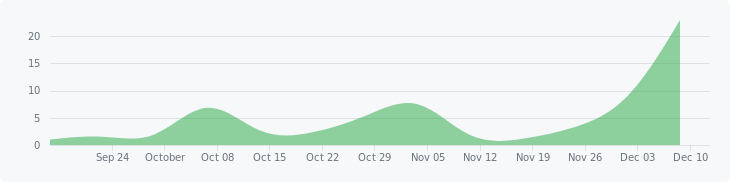
\includegraphics[width=\linewidth]{pics/contributions.png}
%    \caption{Beiträge in der Dokumentations-Ablage auf GitHub im Herbstsemester 2017\label{fig:contributions}}
%\end{figure}

